\documentclass{beamer}
\usetheme{default}
\usecolortheme{default}

%% custom color theme. 
\definecolor{sidebartop}{RGB}{133,135,86}
\definecolor{sidebar}{RGB}{177,179,115}
\definecolor{sidebarbot}{RGB}{211,213,136}
\definecolor{title}{RGB}{241,243,186}
\setbeamertemplate{sidebar canvas left}[vertical shading][top=sidebar,bottom=sidebarbot]
\setbeamercolor{frametitle}{fg=title,bg=sidebar}
\setbeamercolor{logo}{fg=sidebar,bg=sidebar}
\setbeamercolor{sidebar}{fg=sidebarbot}
\setbeamercolor{title in sidebar}{fg=title}
\setbeamercolor{author in sidebar}{fg=title}
\setbeamercolor{section in sidebar}{fg=white}
\setbeamercolor{section in sidebar shaded}{fg=title}
\setbeamercolor{item}{fg=sidebar}

%%%%%%%%%%%%%%%%%%
%% For printing handout
%\documentclass[handout]{beamer}
%\usepackage{pgfpages}
%\pgfpagesuselayout{2 on 1}[letterpaper,border shrink=10mm]
%%\pgfpageslogicalpageoptions{1}{border code=\pgfusepath{stroke}}
%%\pgfpageslogicalpageoptions{2}{border code=\pgfusepath{stroke}}
%\usetheme{default}
%\usecolortheme{default}
%% Handout commands end here
%%%%%%%%%%%%%%%%%%

\usepackage{color}
\usepackage{graphicx}

\usepackage[lined]{algorithm2e}

%\usepackage{bibentry}
%\nobibliography*
\begin{document}
{
\usebackgroundtemplate{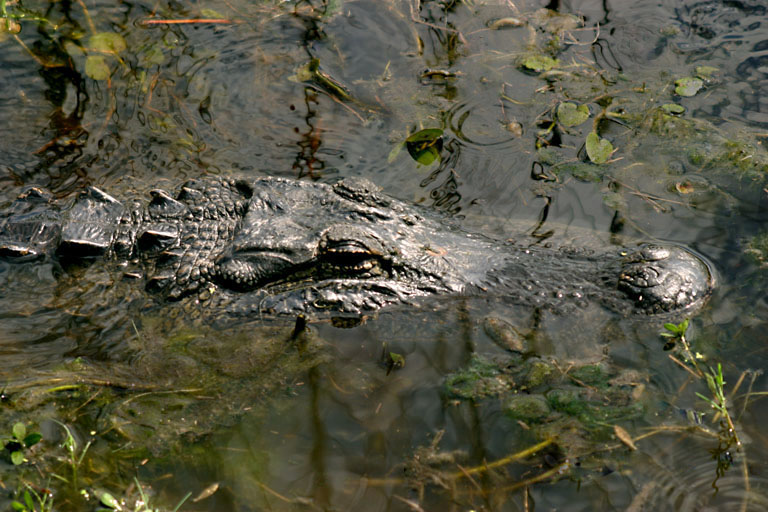
\includegraphics[height=\paperheight]{figure/GatorHeadModified.jpg}}
\begin{frame}[plain,c]
% \vspace*{-0.1in}
\begin{center}
  {\color[RGB]{241,243,186}
{\huge EEL6935 Course Project Proposal}\\
  \vspace*{1.8in}
{\bf presenter's name}, name, name \\
    \vspace*{1em}
  \begin{tabular}{cc}
  University of Florida
   \end{tabular}
}
  \end{center}
\hoffset=0em
\end{frame}}

\begin{frame}
\frametitle{test}
test frame
\end{frame}

\end{document}
